\section{Question 3}



\subsection{Testing the hypothesis}

The following hypothesis has been established based on the findings in Questions~1 and 2:
It is theoretically possible for the Scottish electricity grid to be independent and meet its electricity demand of 35,810~GWh with 100\% RE generation if:
\begin{itemize}
	\item The current RE generation mix is scaled up by 36.4\%, as shown in Table~\ref{tbl:upscale}
	\item There is PHS of 75\% efficiency with a power rating of 3.43~GW and a storage period of at least three days
\end{itemize}

EnergyPLAN was used to test this hypothesis.
To get a storage period of at least three days, 240~GWh was selected as the PHS storage capacity for a couple reasons.
Firstly, at a power rating of 3.43~GWh (to meet the peak power demand), a PHS scheme of 240~GWh storage capacity can operate continuously for about three days before the reservoirs are depleted.
Secondly, it is assumed the grid would not need to meet Scotland's peak power demand continuously for three days.
Therefore, if it is possible to limit the PHS power rating to 1.43~GW (to meet the mean winter demand), 240~GWh would yield a storage period of one week.



\subsubsection{EnergyPLAN inputs}

EnergyPLAN's UK 2020 model \citep{EnergyPLAN_UK2020} was used as the baseline for the hypothesis.
It contained distribution files with hourly data for a year that described typical weather and energy generation patterns etc.
Some of default data inputs were amended so that there was only an electricity demand of 35.81~TWh/ year (and no heating, cooling or transport demand etc.), only RE generation (so no heat supply from district heating, combined heat and power (CHP) or heat pumps etc.) and no transmission line capacity (see Figure~\ref{fig:B02-base_load}).
Additionally, the minimum grid stabilisation production share (MGSPS) was set to 30\%, as recommended by the EnergyPLAN manual \citep{Lund2017}.

Figure~\ref{fig:B02-base_load} shows the \textbf{base load} inputs.
The upscaled large scale hydro capacity of 1,829~MW was entered for Dammed Hydro Power.
The default Dammed Hydro Power efficiency was left untouched and, instead, the water supply to the Dammed Hydro was amended until the estimated annual production equalled the upscaled large scale hydro generation calculated in Question~1, i.e. 6.12~TWh/ year (see Table~\ref{tbl:upscale}).

``Condensing PP2" consists of the central power plants that generate electricity only.
PP2 was allocated 570~MW, i.e. the upscaled capacity of landfill gas, sewage sludge digestion and other biomass (see Section~\ref{sec:base_load}).
The electrical efficiency of landfill gas, sewage sludge digestion and biomass energy generation were respectively found as 42\% \citep{ClarkeEnergy}, 15\% \citep{Mills2015} and 25\% \citep{BERC2009}.
The average, 27\%, was entered as the efficiency of PP2.

Figure~\ref{fig:B01-BM} shows the \textbf{distribution of resources that fuel the power plants} in EnergyPLAN.
For the purposes of this exercise, PP2 was the only plant that was used, and biomass represented landfill gas, sewage sludge digestion and other biomass.
The annual amount of biomass supply was calculated by dividing the upscaled generation of the individual RE generators by their respective efficiencies, and then by summing the quotients (see Table~\ref{tbl:BM_supply_calc}).
The sum, 11.529~TWh, was entered into EnergyPLAN.

\begin{table}[htbp]
	\caption{Calculation of annual biomass fuel supply to PP2.}
	\label{tbl:BM_supply_calc}
	\centering
	\begin{tabular}{@{}lrrr@{}}
		\toprule
		Dispatchable load & Upscaled generation (TWh) & Efficiency & PP2 fuel consumption (TWh) \\ \midrule
		Landfill gas & 0.69 & 42\% & 1.650 \\
		Sewage sludge digestion & 0.04 & 15\% & 0.268 \\
		Other biomass & 2.40 & 25\% & 9.612 \\ \midrule
		Total & 3.14 & -- & 11.529 \\ \bottomrule
	\end{tabular}
\end{table}

The installed capacities of the upscaled \textbf{variable renewable electricity (VRE) mix}, which were calculated in Table~\ref{tbl:upscale}, were entered into EnergyPLAN as shown in Figure~\ref{fig:B02-VRE}.
The correction factors were tweaked so that the estimated post correction production (in TWh/year) equalled the upscaled generation calculated in Table~\ref{tbl:upscale}.

The \textbf{PHS parameters}, e.g. the 240~GWh storage capacity, were entered as shown in Figure~\ref{fig:B02-PHS}.
The pump and turbine efficiencies at a PHS facility are typically the same.
Inserting a pump and turbine efficiency of 86.61\% gives the desired round-trip efficiency of $0.8661 \times 0.8661 = 0.75$ \citep{Connolly2015}.

Moreover, the turbine and pump were allowed for simultaneous operation to better integrate fluctuating RE generation.
This is unlike traditional PHS facilities (described in Section~\ref{sec:PHS}).
Traditional facilities must either prioritise the pump or turbine.
If the pump is prioritised, excess electricity gets stored while other power plants are left to supply grid-stabilising power.
%Such a system often requires more fuel
% which work on a daily cycle, charging at night and discharging in the day; these were either unable or had no need to use the pump and turbine simultaneously.
However, operating the pump and turbine together enables the PHS scheme to store excess VRE while also producing grid-stabilising power.
This can be achieved with a double penstock set-up, as shown in Figure~\ref{fig:penstock_systems}, or ``by installing multiple single penstock system [PHS] facilities on the same energy system i.e. one can charge while the other is discharging at the same time" \citep[p.~39]{Connolly2015}.
Because the PHS storage capacity does not replenish as quickly with a double penstock system, it also allows for lower storage capacities than single penstock systems \citep{Connolly2015}.

\begin{figure}[htbp]
	\centering
	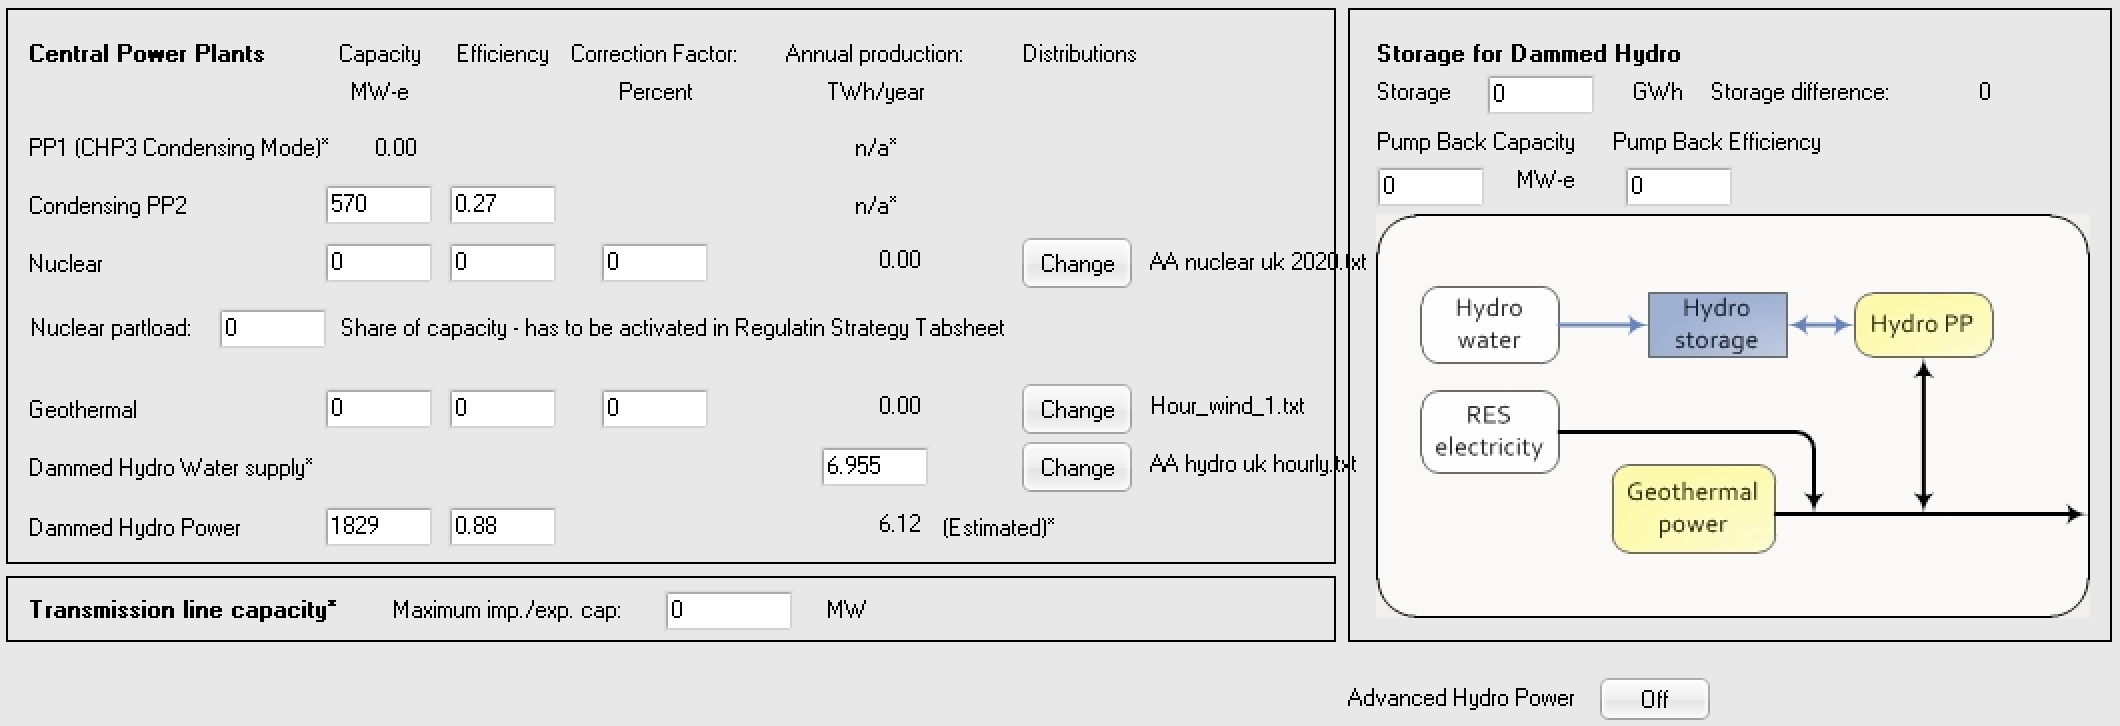
\includegraphics[width=\textwidth]{figures/B02_base_load.png}
	\rule{\textwidth}{0.5pt} % use line???
	\caption{Base load parameters and nullified transmission line capacity (screenshot of EnergyPLAN).}
	\label{fig:B02-base_load}
\end{figure}

\begin{figure}[htbp]
	\centering
	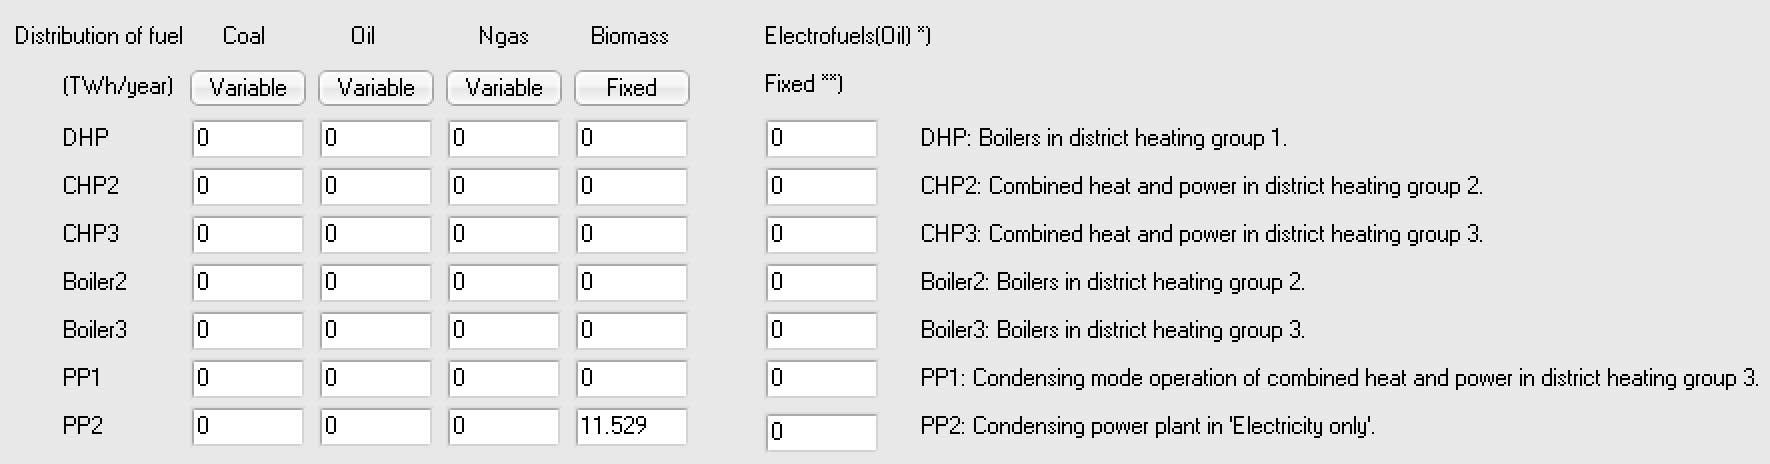
\includegraphics[width=\textwidth]{figures/B01_BM.png}
	\rule{\textwidth}{0.5pt} % use line???
	\caption{Initial supply of biomass to PP2 (screenshot of EnergyPLAN).}
	\label{fig:B01-BM}
\end{figure}

\begin{figure}[htbp]
	\centering
	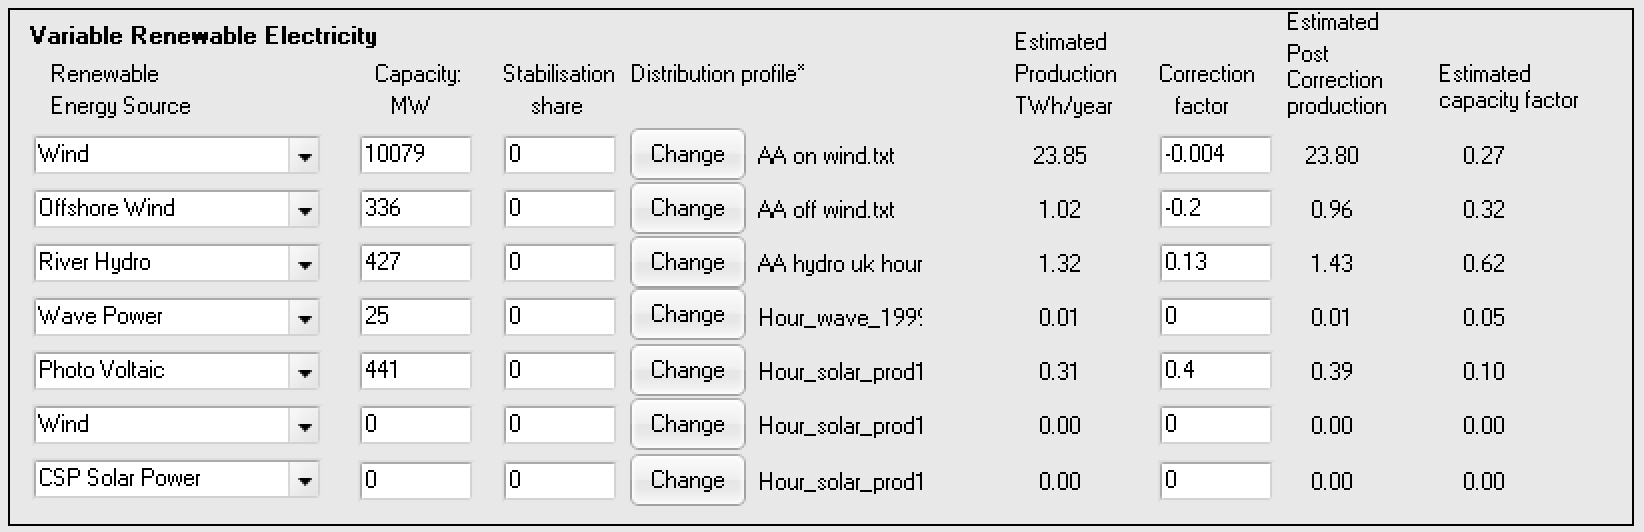
\includegraphics[width=\textwidth]{figures/B02_VRE.png}
	\rule{\textwidth}{0.5pt} % use line???
	\caption{VRE generation mix (screenshot of EnergyPLAN).}
	\label{fig:B02-VRE}
\end{figure}

\begin{figure}[htbp]
	\centering
	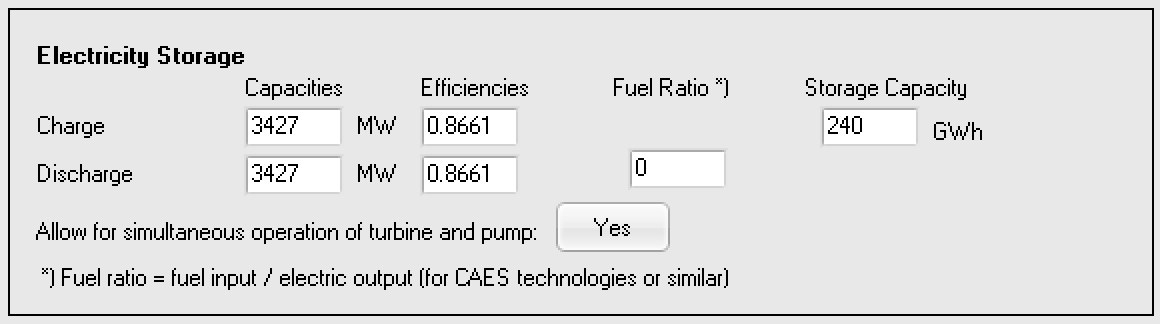
\includegraphics[width=\textwidth]{figures/B02_PHS.png}
	\rule{\textwidth}{0.5pt} % use line???
	\caption{PHS parameters.}
	\label{fig:B02-PHS}
\end{figure}

\begin{figure}[htbp]
	\centering
	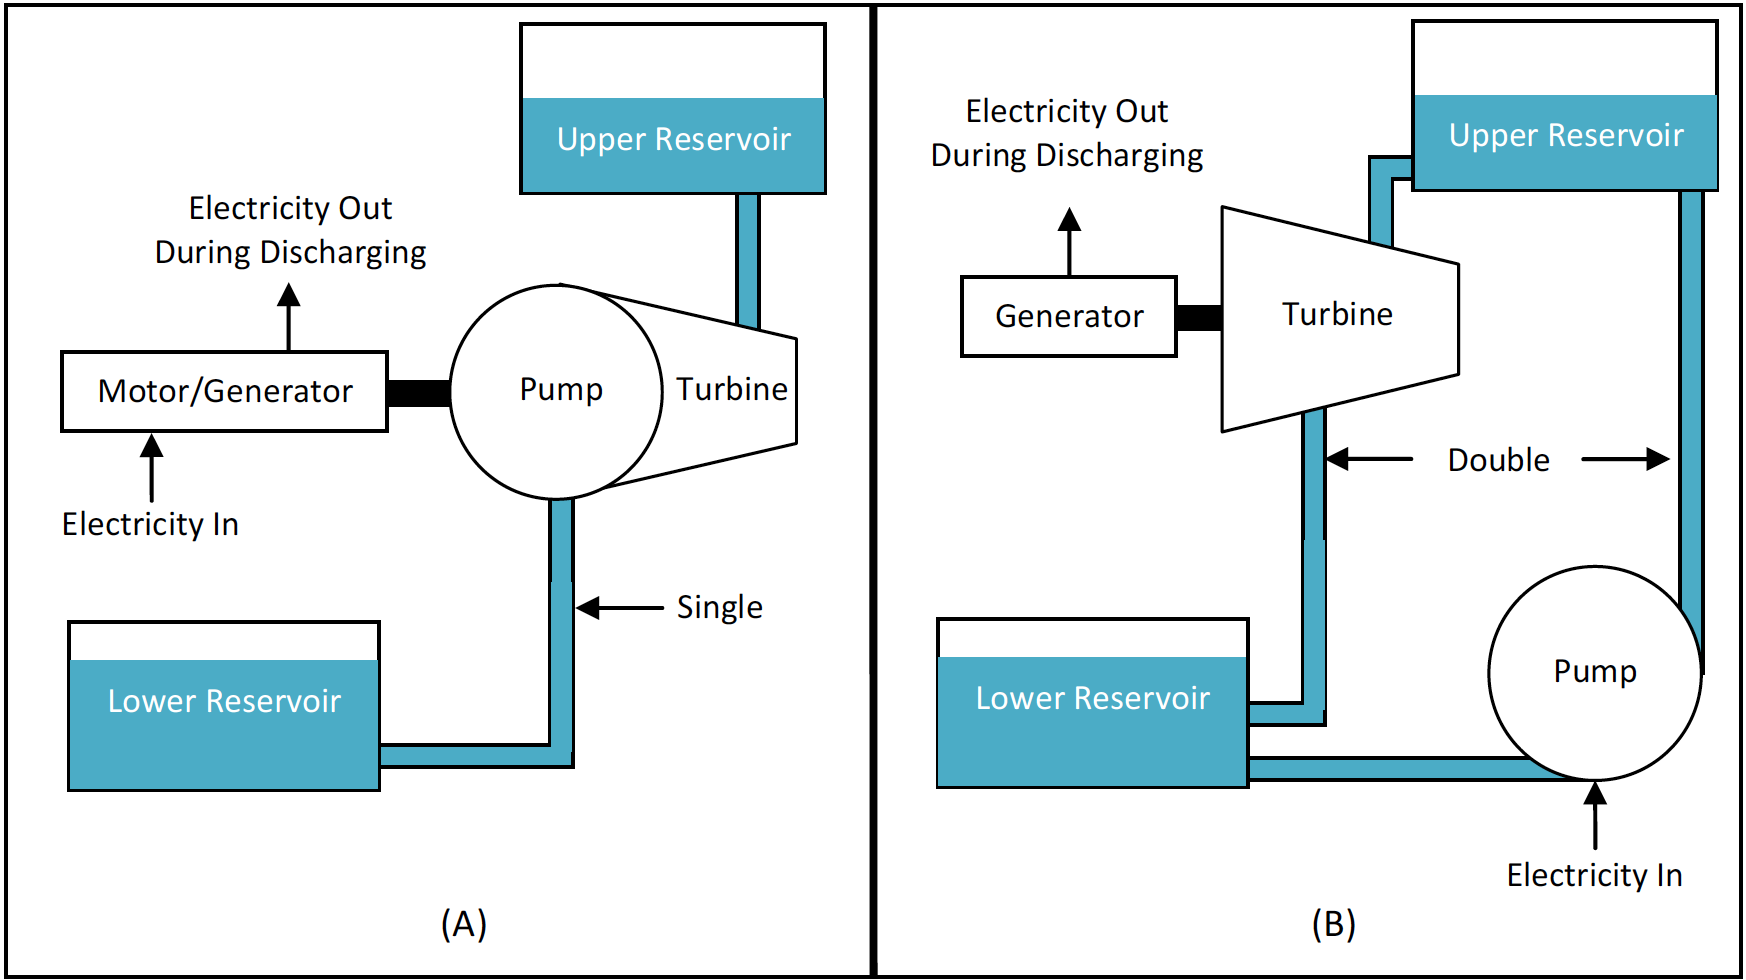
\includegraphics[width=\textwidth]{figures/penstock_systems.png}
	\rule{\textwidth}{0.5pt} % use line???
	\caption{PHS with (A) a single penstock system and (B) a double penstock system \citep[p.~39]{Connolly2015}.}
	\label{fig:penstock_systems}
\end{figure}



\subsubsection{Hypothesis evaluation}

The initial run of the hypothetical scenario in EnergyPLAN triggered the ``(1) Critical Excess", ``(2) Grid Stab. Problem" and ``(3) PP/Import problem" warnings.
The exports and imports are displayed in Figure~\ref{fig:B15_balance}.
It was also noticed that the programme deemed the specified biomass fuel supply insufficient, so it added 0.96~TWh/year of fuel, 75\% of which was fossil.

The grid stability load fluctuated between 61\% and 320\% in the simulated year.
The grid is not stable when the grid stability load is below 100\% at any given time of the year.
The grid was not stable because at least one time in the simulated year, the grid stabilisation technologies (PP2, dammed hydro and PHS) generated less than the required amount specified by the MGSPS, i.e. 30\%.
This means that more than 70\% of the electricity was VRE during these times.
When the stabilisation load is greater than 100\%, it means that more grid stabilisers had to be used to meet the demand, probably because there wasn't enough VRE generation.
Moreover, the fact that the annual average of the stabilisation load was 159\% indicates that there was not enough VRE generation.

The scenario was re-run with a MGSPS of 15\% and the first Critical Electricity Excess Production (CEEP) regulation, i.e. reducing RES1 and RES2.
The latter measure essentially curtails the onshore and offshore wind production when it exceeds the demand.
Together, these two measures got rid of the ``(1) Critical Excess" and ``(2) Grid Stab. Problem" warnings.
However the ``(3) PP/Import problem" still remained.
The lack of exports and remainder of imports, though seemingly less frequent, is seen in Figure~\ref{fig:B14_balance}.
It was also noticed that, in the amended scenario, less fuel was needed for PP2.
Despite a biomass supply of 11.529~TWh/year being specified, only 10.78~TWh/year of biomass was used/ needed.

\begin{figure}[htbp]
    \centering
        \begin{subfigure}{.48\textwidth}
          \centering
          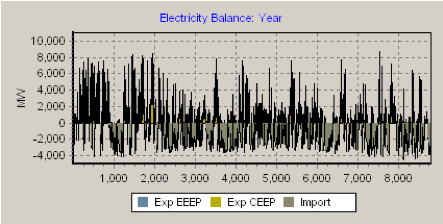
\includegraphics[width=\textwidth]{figures/B15_balance.png}
%          \rule{\textwidth}{0.5pt} % use line???
          \caption{Initial run}
          \label{fig:B15_balance}
        \end{subfigure}
        \begin{subfigure}{.48\textwidth}
          \centering
          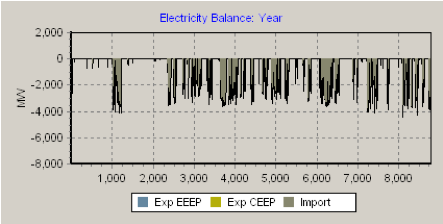
\includegraphics[width=\textwidth]{figures/B14_balance.png}
%          \rule{\textwidth}{0.5pt} % use line???
          \caption{After CEEP and MGSPS amendments}
          \label{fig:B14_balance}
        \end{subfigure}
    \rule{\textwidth}{0.5pt} % use line???
    \caption{Annual electricity balance graphs showing imports and exports for the tested hypothetical scenario in EnergyPLAN.}
    \label{fig:B15_B14_balance}
\end{figure}

Flexible demand...

The ``(3) PP/Import problem" warning could not go away without increasing the base load and/ or VRE capacity which, for the sake of the hypothesis, had to stay fixed.
Hence, the hypothesis was proven to be false, mainly because the upscaled RE generation mix could often not meet the demand.




\subsection{Scenario optimisation}


